\documentclass{report}
\usepackage{makeidx}
\usepackage{graphicx}
\usepackage{subfigure}
\usepackage{titlesec}
\usepackage{fullpage}
\setcounter{secnumdepth}{4}
\usepackage[utf8]{inputenc}
\usepackage{import}
\usepackage{doxygen}
\usepackage{hyperref}
\usepackage{amsmath,diagbox,ifthen}

\title{HZCC Developer Guide}
\author{Hanze Chen}
\date{}
\makeindex

%% doxygen fix
\newcommand{\+}{}


\begin{document}
    \maketitle


    \chapter{Compiler frontend}
    \section{Introduction}\label{sec:introduction}
    The following diagram, numbered modes, examples and token tables describe
    the January 2022 coursework. For the current command line, see
    Section~\ref{sec:user-manual}. For the current token numbers, see
    \path{hzcc/parser/common/token_type.h}.
    \begin{figure}[hb!]
        \centering
        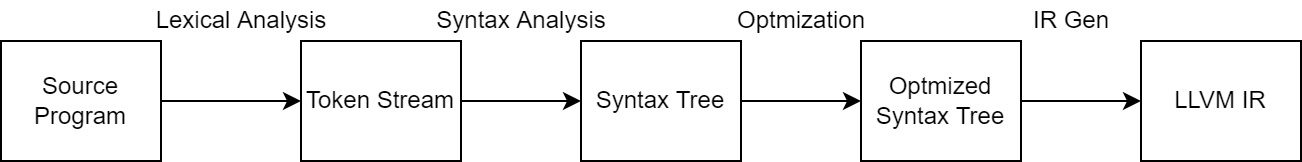
\includegraphics[width=10cm]{figure/frontend_structure}
        \caption{Frontend Structure}
        \label{fig:frontend_structure}
    \end{figure}


    \section{Implemented Function}\label{sec:implemented-function}

    \subsection{Part0}\label{subsec:part0}
    The coursework used \verb|-0| to request the version banner shown in
    Figure~\ref{fig:example_part0_output}.
    \begin{figure}[hb!]
        \centering
        \fbox{
            \shortstack[l]{
                My bare-bones C compiler (for COM 440/540) \\
                Written by Hanze Chen (hanzech@iastate.edu) \\
                Version 0.1.0\_9c370c3(WorkStation) \\
                2022-01-28 13:18:14
            }
        }
        \caption{Example Output for Part 0}
        \label{fig:example_part0_output}
    \end{figure}

    CMake supplied the version, commit hash, build hostname and build time through
    the generated \verb|version.h| header. The assignment allowed \verb|-o| to
    redirect the banner. The current \verb|--version| option writes to stdout.

    \subsection{Part1}\label{subsec:part1}
    The original \verb|-1| mode listed tokens on stdout or in the file selected
    with \verb|-o|. Each row identified a source file, a line, a numeric token
    category and its spelling. Figure~\ref{fig:example_part1_output} shows the
    original output for \verb|hello.c|. Table~\ref{tab:tokens} gives the
    coursework token numbers.

    \begin{quote}
        \texttt{File} \emph{filename} \texttt{Line} \emph{line number}
        \texttt{Token} \emph{token number} \texttt{Text} \emph{lexeme}
    \end{quote}

    The original diagnostic format placed the location and offending text on
    the first line of stderr, followed by the description on the second line.

    \begin{quote}
        \texttt{Lexer error in file} \emph{filename} \texttt{line}
        \emph{line number} \texttt{near text} \emph{lexeme}\\
        \hspace*{1em}\emph{Description}
    \end{quote}

    \begin{figure}[hb!]
        \centering
        \fbox{
            \shortstack[l]{
                File hello.c Line 8 Token 301 Text int\\
                File hello.c Line 8 Token 306 Text main\\
                File hello.c Line 8 Token 40 Text (\\
                File hello.c Line 8 Token 41 Text )\\
                File hello.c Line 9 Token 123 Text \{\\
                File hello.c Line 10 Token 410 Text return\\
                File hello.c Line 10 Token 306 Text printf\\
                File hello.c Line 10 Token 40 Text (\\
                File hello.c Line 10 Token 305 Text "Hello, world!"\\
                File hello.c Line 10 Token 41 Text )\\
                File hello.c Line 10 Token 59 Text ;\\
                File hello.c Line 11 Token 125 Text \}
            }
        }
        \caption{Part1 example output}
        \label{fig:example_part1_output}
    \end{figure}


    \subsection{Part3}\label{subsec:part3}
    The original \verb|-3| mode checked the input file's syntax. The assignment
    required the first syntax error to identify the filename, line and offending
    token on stderr, followed by a description of what the parser expected.
    The legacy syntax fixtures check this format.

    \begin{quote}
        \texttt{Parser error in file} \emph{filename} \texttt{line}
        \emph{line number} \texttt{near text} \emph{lexeme}\\
        \hspace*{1em}\emph{Description}
    \end{quote}

    On success the assignment expected the following line.

    \begin{quote}
        \verb|File| \emph{filename} \verb|is syntactically correct.|
    \end{quote}

    The assignment used the following operator precedence and associativity.
    \begin{table}[t]
        \begin{center}
            \begin{tabular}{@{}l|c|c}
                \hline
                \multicolumn{1}{c|}{\sc Operators}
                &
                    {\sc Associativity}
                &
                    {\sc Precedence}
                \\ \hline
                \verb|()| \quad \verb|[]| \quad .
                &
                left to right
                &
                (highest)
                \\
                \verb|!| \quad \verb|~| \quad \verb|-| (unary)
                \quad \verb|--| \quad \verb|++|
                % \quad \verb|&| (unary)
                \quad \verb|(|\emph{type}\verb|)|
                &
                right to left
                \\
                \verb|*| \quad \verb|/| \quad \verb|%|
                &
                left to right
                \\
                \verb|+| \quad \verb|-|
                &
                left to right
                \\
                \verb|<| \quad \verb|<=| \quad \verb|>| \quad \verb|>=|
                &
                left to right
                \\
                \verb|==| \quad \verb|!=|
                &
                left to right
                \\
                \verb|  &  |
                &
                left to right
                \\
                \verb$|$
                &
                left to right
                \\
                \verb|  &   &  |
                &
                left to right
                \\
                \verb$||$
                &
                left to right
                \\
                \verb$?:$
                &
                right to left
                \\
                \verb|=| \quad \verb|+=| \quad \verb|-=| \quad \verb|*=| \quad \verb|/=|
                &
                right to left
                \\
                \verb|,|
                &
                left to right
                &
                (lowest)
                \\ \hline
            \end{tabular}
        \end{center}
        \caption{Precedence and associativity of operators}
        \label{TAB:precedence}
    \end{table}


    \section{Component}\label{sec:component}

    \subsection{lexical}\label{subsec:lexical}
    Table~\ref{tab:tokens} lists the coursework token numbers for punctuation,
    operators, keywords and tokens carrying a source spelling.
    \begin{table}[t]
        \centering
        \begin{tabular}{rlcrlcrl}
            \multicolumn{8}{c}{Single character symbols}
            \\[1mm]
            {\bf Value} & {\bf Lexeme}
            & ~~~~~~ &
                {\bf Value} & {\bf Lexeme}
            & ~~~~~~ &
                {\bf Value} & {\bf Lexeme}
            \\ \cline{1-2} \cline{4-5} \cline{7-8}
            33 & \verb|!| & &
            37 & \verb|%| & &
            38 & \verb|  &  | \\
            40 & \verb|(| & &
            41 & \verb|)| & &
            42 & \verb|*| \\
            43 & \verb|+| & &
            44 & \verb|,| & &
            45 & \verb|-| \\
            46 & \verb|.| & &
            47 & \verb|/| & &
            58 & \verb|:| \\
            59 & \verb|;| & &
            60 & \verb|<| & &
            61 & \verb|=| \\
            62 & \verb|>| & &
            63 & \verb|?| & &
            91 & \verb|[| \\
            93 & \verb|]| & &
            123 & \verb|{| & &
            124 & \verb+|+ \\
            125 & \verb|}| & &
            126 & \verb|~| \\
            \\
            \multicolumn{8}{c}{Operators with two characters}
            \\[1mm]
            {\bf Value} & {\bf Lexeme}
            & ~~~~~~ &
                {\bf Value} & {\bf Lexeme}
            & ~~~~~~ &
                {\bf Value} & {\bf Lexeme}
            \\ \cline{1-2} \cline{4-5} \cline{7-8}
            351 & \verb|==| & &
            352 & \verb|!=| & &
            353 & \verb|>=| \\
            354 & \verb|<=| & &
            355 & \verb|++| & &
            356 & \verb|--| \\
            357 & \verb+||+ & &
            358 & \verb|&  &  | & &
            361 & \verb|+=| \\
            362 & \verb|-=| & &
            363 & \verb|*=| & &
            364 & \verb|/=| \\
            \\
            \multicolumn{8}{c}{keywords}
            \\[1mm]
            {\bf Value} & {\bf Lexeme}
            & ~~~~~~ &
                {\bf Value} & {\bf Lexeme}
            & ~~~~~~ &
                {\bf to\_str} & {\bf Lexeme}
            \\ \cline{1-2} \cline{4-5} \cline{7-8}
            401 & \verb|const| & &
            402 & \verb|struct| & &
            403 & \verb|for| \\
            404 & \verb|while| & &
            405 & \verb|do| & &
            406 & \verb|if| \\
            407 & \verb|else| & &
            408 & \verb|break| & &
            409 & \verb|continue| \\
            410 & \verb|return| & &
            411 & \verb|switch| & &
            412 & \verb|case| \\
            413 & \verb|default| \\
        \end{tabular}

        \begin{tabular}{rll}
            \\
            \multicolumn{3}{c}{Lexemes with attributes}
            \\[1mm]
            {\bf Value} & {\bf Lexeme} & {\bf Definition}
            \\ \hline
            301 & type & \verb|void| or \verb|char| or \verb|int| or \verb|float|
            \\
            302 & character literal & a character enclosed in single quotes;
            escape sequences are extra credit
            \\
            303 & kInt literal & a sequence of one or more digits
            \\
            304 & real literal & two sequences each of one or more digits, separated by \verb|.|
            \\
            305 & string literal & a sequence of zero or more characters (including escape sequences,
            \\ & & except for \verb|\\| and \verb|\"|) enclosed in double quotes
            \\
            306 & identifier & a letter or underscore, followed by zero or more letters,
            underscores, or
            \\ & & digits, that is not a keyword or type
        \end{tabular}

        \caption{Tokens to be recognized by the lexer.}
        \label{tab:tokens}
    \end{table}


    \section{Main Data Structures}\label{sec:main-data-structures}

    \subsection{lexical}\label{subsec:lexical2}

    \subsubsection{StringToken \index{String Token Class}}
    In the original frontend diagram (Figure~\ref{fig:frontend_structure}),
    a \verb|TokenStream| held the source file's \verb|StringToken| objects.
    Table~\ref{tab:supported_lexical_token_list} lists their lexical patterns.
    \begin{table}[hb!]
        \centering
        \begin{tabular}{l|lll}
            \hline
            Token type   & Regex                                                  & Example           & Description    \\ \hline
            Add          & \textbackslash{}\textbackslash{}+                      & +                 & Addition       \\
            Sub          & -                                                      & -                 & Subtraction    \\
            Mul          & \textbackslash{}\textbackslash{}*                      & *                 & Multiplication \\
            Div          & /                                                      & /                 & Division       \\
            Mod          & \%                                                     & \%                & Modulus        \\
            Assign       & =                                                      & =                 & Assignment     \\
            Exclamatory  & !                                                      & !                 & Exclamation    \\
            LBracket     & \textbackslash{}\textbackslash{}(                      & (                 & Left Bracket   \\
            RBracket     & \textbackslash{}\textbackslash{}(                      & )                 & Right Bracket  \\
            LBrace       & \textbackslash{}\{                                     & \{                & Left Brace     \\
            RBrace       & \textbackslash{}\}                                     & \}                & Right Brace    \\
            Comma        & ,                                                      & ,                 & Comma          \\
            Semicolon    & ;                                                      & ;                 & Semicolon      \\
            Colon        & :                                                      & :                 & Colon          \\
            Dot          & \textbackslash{}\textbackslash{}.                      & .                 & Dot            \\
            Greater      & \textgreater{}                                         & \textgreater{}    & Greater        \\
            LT         & \textless{}                                            & \textless{}       & LT           \\
            LBound       & \textbackslash{}[                                      & {]}               & Left Bound     \\
            RBound       & \textbackslash{}]                                      & {[}               & Right Bound    \\
            QuestionMark & \textbackslash{}\textbackslash{}?                      & ?                 & Question Mark  \\
            Esperluette  & \textbackslash{}\&                                     & \&                & Esperluette    \\
            Star         & \textbackslash{}\textbackslash{}*                      & *                 & Star           \\
            VerticalBar  & \textbackslash{}\textbackslash{}|                      & |                 & Vertical Bar   \\
            number       & {[}0-9{]}+\textbackslash{}\textbackslash{}.?{[}0-9{]}* & 0, 0.1 etc.       & Numbers        \\
            Identifiers  & {[}a-zA-Z\_{]}{[}a-zA-Z0-9\_{]}*                       & "a", "while" etc. & Identifiers    \\ \hline
        \end{tabular}
        \caption{Supported String Token type}
        \label{tab:supported_lexical_token_list}
    \end{table}

    \subsection{Utils}\label{subsec:utils}

    \subsubsection{Status \index{Status Class}}
    Frontend stages return \verb|hzcc::Status| for an operation and
    \verb|hzcc::StatusOr<T>| when a successful operation also produces a value.
    The current interfaces live in \path{hzcc/utils/status/}.


    \section{User Manual}\label{sec:user-manual}
    HZCC is an experimental C compiler written in C++17. The default build runs
    a handwritten lexer and parser. Each invocation accepts multiple source files
    and at most one analysis mode. The following commands assume a Debug build.

    \begin{verbatim}
build/debug/bin/hzcc --version
build/debug/bin/hzcc --flexical_only test/lexical/hello.c
build/debug/bin/hzcc --fsyntax_only source.c
    \end{verbatim}

    Lexical mode prints tokens in input order. To save the combined listing, pass
    \verb|-o| with a writable path. Quote paths that contain spaces. The driver
    opens the destination after all inputs pass lexical analysis and reports
    write errors. Syntax mode prints a success message for each accepted file.
    A syntax error returns status 1 and a lexical error returns status 4.
    Only lexical mode accepts \verb|-o|. Use \verb|--fno_color| for plain-text
    diagnostics. Syntax errors identify the unexpected token. If the source can
    be read, the compiler shows its line and marks the token with a caret. A
    conflicting function prototype reports the previous and current types.

    \clearpage
    \appendix


    \part*{API reference}
    \subimport{latex/}{refman.tex}

    \printindex
\end{document}
